\subsection{Measurements}\label{sec:cloud:crowdsourcing:measurements}
In this section we analyse a large dataset from a commercial crowdsourcing platform to derive to derive realistic model parameters and compare the model based on these results with the analytic approximation.

\subsubsection*{Deriving Realistic Model Parameters}
Our analysis is based on a large dataset from the commercial micro-tasking platform Microworkers.com.
The dataset contains information about more then 160.000 campaigns submitted to the platform between May 2009 and Jan 2015, including the number of task per campaign was well as the time of the submission of the campaign.  

\paragraph*{Inter-arrival Times:} First, we study the inter-arrival times of the campaigns.
During the observation period, the platform faced some downtime due to software update or changes of the technical infrastructure.
During this time, no campaigns could be submitted resulting in relatively large campaign inter-arrival times.
In our model we only consider the regular operation of the platform, therefore we removed all inter-arrival times larger then \SI{97.5}{\percent} quantile of all observed values, which affects about \SI{2.5}{\percent} of all values.

\begin{figure}
  \centering
  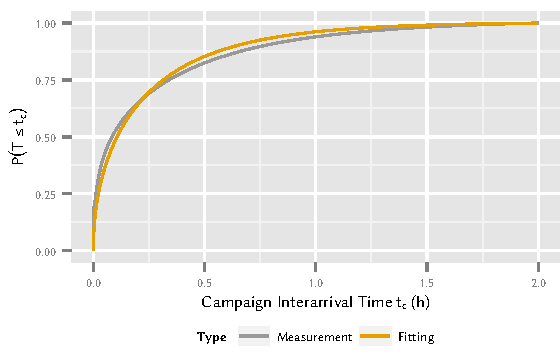
\includegraphics{cloud/crowdsourcing/measurements/figures/campaign_interarrival}
  \caption{Observed campaign inter-arrival times \(t_c\) and corresponding fit.}
  \label{fig:cloud:crowdsourcing:measurements:parameters:campaign_interarrival}
\end{figure}

Considering the remaining data, we observe a mean campaign inter-arrival time of \SI{0.241}{\hour} with a standard deviation \SI{0.346}{\hour}.
\reffig{fig:cloud:crowdsourcing:measurements:parameters:campaign_interarrival} shows the \gls{CDF} of considered inter-arrival times, as well as the fitted distribution.
For the fitting we considered several possible distributions but found the gamma distribution 

\[
P(t_c=t) \sim \Gamma(\alpha,\beta,t_c) = \frac{\beta^\alpha}{\Gamma(\alpha)} x^{\alpha-1} e^{-{\beta}t_c}
\]

defined by shape \(\alpha\) and rate \(\beta\) to be the most suitable.
Using \texttt{fitdistrplus}\footnote{\url{https://cran.r-project.org/web/packages/fitdistrplus}, \accessed} for the R language we derive the distribution parameters for the campaign inter-arrival times \(\campaignIAT\) by moment fitting and result in the estimated parameters \(\alpha=0.484\) and \(\beta=2.009\).

\paragraph*{Campaign Sizes:}Next, we consider the campaign sizes, respectively the number of tasks per campaign.
The smallest possible campaign sizes on Microworkers is \(30\) tasks, however our dataset contained a few internal test campaigns with a small size.

These test campaigns, as well as outliers larger than the \SI{97.5}{\percent} quantile of the campaign size have been removed from the considered dataset.
In total \SI{3.7}{\percent} of the original dataset were filtered by these conditions, the remaining data resulted in a mean campaign size of \(97.01\) tasks and a standard deviation of \(103.41\).
The \gls{CDF} of the campaign sizes \campaignSize is depicted in \reffig{fig:cloud:crowdsourcing:measurements:parameters:campaign_sizes}, together with the corresponding fitted distribution.

\begin{figure}
  \centering
  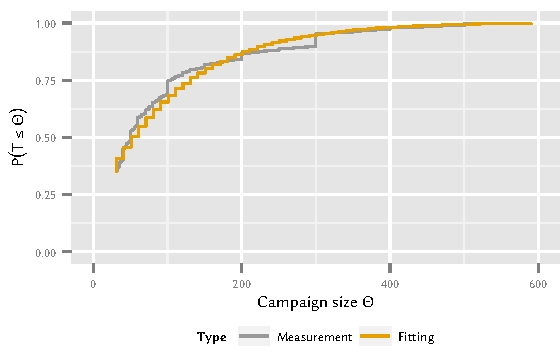
\includegraphics{cloud/crowdsourcing/measurements/figures/campaign_sizes}
  \caption{Observed campaign sizes \campaignSize and corresponding fit.}
  \label{fig:cloud:crowdsourcing:measurements:parameters:campaign_sizes}
\end{figure}

Due to the platform restrictions mentioned above, the campaign sizes start with a minimum value of \(30\) tasks.
We observer that a very high share, i.e. \SI{35}{\percent}, of campaigns has only this minimum size.
Further, campaign sizes which are a multiple of ten or a multiple of \(100\) are quite frequent.
This is caused by the fact that most task on Microworkers.com are repetitive and the employers choose the required number of repetitions and thus are more likely to round the number of repetitions to the nearest multiple of ten or \(100\).

In order to obtain an suitable analytic distribution for the empiric values, we divided the observed values and use the following piecewise defined distribution.
\begin{equation*}
P(S=s) \sim
\begin{cases}
  0 & \text{if } s < s_{\min}\\
  p_{s_{\min}} & \text{if } s=s_{\min} \\
  GEOM(s) \cdot 10 + (s_{\min}+1) & \text{else}
\end{cases}
\end{equation*}
with 
\begin{equation*}
GEOM(s) = {(1-p)}^s p
\end{equation*}
The minimum campaign size \(s_{\min}\) is observed with a fixed probability \(p_{s_{\min}}\), while all campaign sizes larger then \(s_{\min}\) follow a shifted and scaled geometric distribution.

Due to the relatively high frequencies of campaign sizes being multiples of \(10\) and \(100\), it is only possible to achieve a good fitting either for the lower or the higher region of the geometric part.
As an overestimation of the campaign size will give us an upper bound of the platform work load, we decided to put a stronger emphasis on correct fitting of the larger campaign sizes.

We estimate the \(p=0.086\) parameter of the geometric distribution using quantile matching for the \SI{90}{percent} quantile.
The values \(s_{\min}=30\) and \(p_{s_{\min}}=0.350\) are obtained from the empirical values.

\paragraph*{Task Duration: }Another relevant model parameter is the length of the tasks \taskDuration, i.e., the time a single worker needs to complete one tasks.
Unfortunately, this information cannot be obtained from our dataset, as tracking of the individual workers is not possible.
Therefore, we assume that the processing times follow a negative-exponential distribution, i.e.
\begin{equation*}
P(t_p=t) \sim \mu  e^{-{\mu}t}
\end{equation*}
Even if the exact processing times are not available, each employer has to add an estimation about the time it task to complete a task in the campaign description.
In our dataset, \SI{87.8}{\percent} of all tasks had an estimated completion time between \SIrange{60}{300}{\second}.
Therefore, we consider \(\mu \in \{\frac{1}{6},\frac{1}{5},\hdots,\frac{1}{2},1\}\) for the following evaluations.

\paragraph*{Number of Workers: }Finally, the last model parameter to estimate is the number of users \numberOfWorkers on the crowdsourcing platform. 
At the time of this analysis, Microworkers.com had over 650.000 registered user accounts.
However, this number is not applicable in the proposed model, for multiple reasons.
The proposed model does not consider vacation times, i.e., the workers would have to be available 24/7.
In reality, many crowdsourcing workers only work occasionally on the platforms or only for a few tasks.
Further, employers can limit the access of to their campaigns to specific subset of all workers, which is also not considered in the model.
Moreover, Microworkers also limits the number of tasks a worker can complete in a single campaign.
Taking this into account, the number of workers to be considered in our model has to be much small then the number of workers on the real world platform and consequently we decided to estimate meaningful values based on the model parameters instead of using the given number of workers from the dataset.

\subsubsection*{Comparison of Detailed and Analytical Model}
An important question for the later analysis is whether the analytic model from \refsec{sec:cloud:crowdsourcing:model} can be used as an approximation or if a simulative evaluation is necessary.
To this end we compared the later considered metrics worker utilisation \workerUtilization and task pre-processing delay \preTaskProcessingDelay for 
\begin{enumerate*}
\item a simulation using the empiric distributions for the task inter-arrival times and campaign sizes,
\item a simulation using the fitted distributions derived earlier in this section, and
\item the analytic model derived in \refsec{sec:cloud:crowdsourcing:model}.
\end{enumerate*}
For the analytical model we used the campaign size distribution derived in this section and \(\lambda=\SI{4.14}{\per\hour}\).
The results of the different models are shown in \reffig{fig:cloud:crowdsourcing:measurements:comparison:distribution}.

\begin{figure*}
	\centering
	\begin{subfigure}{\columnwidth}
		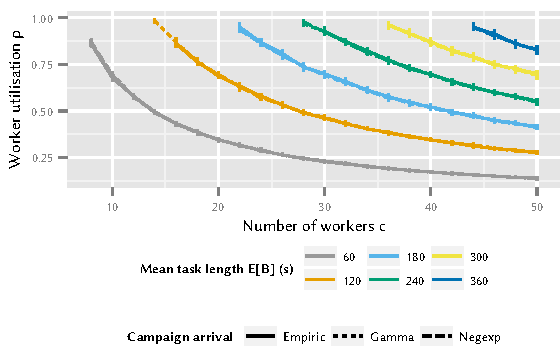
\includegraphics{cloud/crowdsourcing/measurements/figures/distribution_utilization}
		\caption{Worker utilization \workerUtilization}
		\label{fig:cloud:crowdsourcing:measurements:comparison:distribution:utilization}
	\end{subfigure}

	\begin{subfigure}{\columnwidth}
		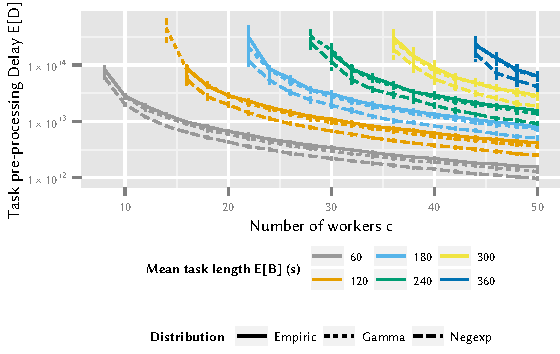
\includegraphics{cloud/crowdsourcing/measurements/figures/distribution_task_delay}
		\caption{Mean task pre-processing delay \preTaskProcessingDelay}
		\label{fig:cloud:crowdsourcing:measurements:comparison:distribution:task_delay}
	\end{subfigure}
	\caption{Comparison of campaign arrival distributions.}
	\label{fig:cloud:crowdsourcing:measurements:comparison:distribution}
\end{figure*}

The worker utilisation \workerUtilization is depicted in \reffig{fig:cloud:crowdsourcing:measurements:comparison:distribution:utilization}, the task pre-processing delay \preTaskProcessingDelay in \reffig{fig:cloud:crowdsourcing:measurements:comparison:distribution:task_delay}.
In both figures, the x-axis shows the number of workers \(\numberOfWorkers\).
The line colour indicates the mean task length, ranging from \SIrange{60}{360}{\second}, the line style denotes the underlying model.
We observe that all models result in the same worker utilisation \workerUtilization, which is not surprising when considering \(\workerUtilization = \frac{E[t_c] E[\campaignSize]}{c\mu}\) with the mean inter-arrival time \(E[t_c]\).
Here, all parameters are the same for the three compared models and therefore, no significant differences can be seen.

This is different for the task pre-processing delay \preTaskProcessingDelay. 
Here, large discrepancies can been observed between the model based on the empiric distributions and the analytical model.
This results show that the \(M^{[\campaignSize]}/M/\numberOfWorkers-\infty\) model can also not be used as a worst case estimations, due to the fact that it underestimates the task pre-processing delay \preTaskProcessingDelay.
In contrast to this, the simulation model based on the gamma distribution fit quite accurate the model based on the empirical values.
Therefore, we decide continue our evaluation with the simulation model, based on the gamma distributed inter-arrival times and the piecewise defined distribution for the campaign sizes.
